\graphicspath{{images/}}

\section{Методы решения обыкновенных дифференциальных уравнений}

\subsection{Решение задачи Коши для ОДУ}

\subsubsection{Постановка задачи}
Реализовать методы Эйлера, Рунге-Кутты и Адамса 4-го порядка в виде программ, задавая в качестве входных данных шаг сетки $h$. С использованием разработанного программного обеспечения решить задачу Коши для ОДУ 2-го порядка на указанном отрезке. Оценить погрешность численного решения с использованием метода Рунге-Ромберга и путем сравнения с точным решением.

\subsubsection{Консоль}
\begin{alltt}
$ make
g++ -g -pedantic -std=c++17 -Wall -Wextra -Werror main.cpp -o solution
$ cat tests/1.in
1 2
2 4 0.1
$ ./solution < tests/1.in
Метод Эйлера:
x = [1.000000, 1.100000, 1.200000, 1.300000, 1.400000, 1.500000, 1.600000, 1.700000, 1.800000, 1.900000, 2.000000]
y = [2.000000, 2.414842, 2.858788, 3.331076, 3.831064, 4.358201, 4.912010, 5.492073, 6.098021, 6.729528, 7.386301]
Погрешность вычислений:
0.000006
Метод Рунге-Кутты:
x = [1.000000, 1.100000, 1.200000, 1.300000, 1.400000, 1.500000, 1.600000, 1.700000, 1.800000, 1.900000, 2.000000]
y = [2.000000, 2.414842, 2.858788, 3.331076, 3.831064, 4.358201, 4.912010, 5.492073, 6.098021, 6.729528, 7.386301]
Погрешность вычислений:
0.000000
Метод Адамса:
x = [1.000000, 1.100000, 1.200000, 1.300000, 1.400000, 1.500000, 1.600000, 1.700000, 1.800000, 1.900000, 2.000000]
y = [2.000000, 2.414842, 2.858788, 3.331076, 3.831062, 4.358197, 4.912005, 5.492067, 6.098015, 6.729521, 7.386294]
Погрешность вычислений:
0.000000
\end{alltt}
\pagebreak

\subsubsection{Результат}
Метод Эйлера
\begin{center}
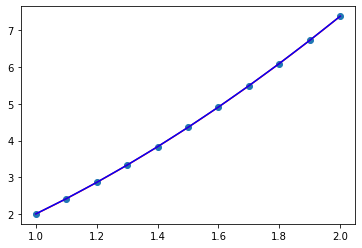
\includegraphics[scale=0.75]{4-1euler}
\end{center}

Метод Рунге-Кутты
\begin{center}
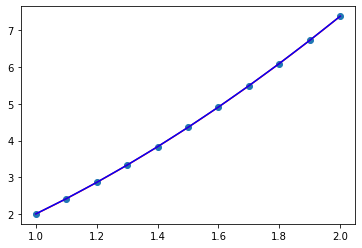
\includegraphics[scale=0.75]{4-1runge}
\end{center}
\pagebreak

Метод Адамса
\begin{center}
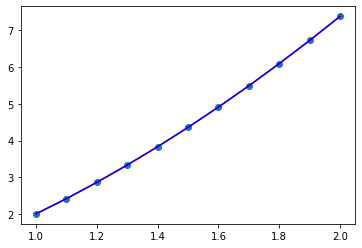
\includegraphics[scale=0.75]{4-1adams}
\end{center}
\pagebreak

\subsubsection{Исходный код}
\lstinputlisting{../lab4_1/simple_desolve.hpp}
\pagebreak

\subsection{Решение краевых задач}

\subsubsection{Постановка задачи}
Реализовать метод стрельбы и конечно-разностный метод решения краевой задачи для ОДУ в виде программ. С использованием разработанного программного обеспечения решить краевую задачу для обыкновенного дифференциального уравнения 2-го порядка на указанном отрезке. Оценить погрешность численного решения с использованием метода Рунге-Ромберга и путем сравнения с точным решением.

\subsubsection{Консоль}
\begin{alltt}
$ make
g++ -g -pedantic -std=c++17 -Wall -Wextra -Werror main.cpp -o solution
$ cat tests/1.in
0.1 0.0001
$ ./solution < tests/1.in
Метод стрельбы:
x = [1.000000, 1.100000, 1.200000, 1.300000, 1.400000, 1.500000, 1.600000, 1.700000, 1.800000, 1.900000, 2.000000]
y = [3.082723, 3.898207, 4.896683, 6.111204, 7.580066, 9.347569, 11.464879, 13.991012, 16.993950, 20.551910, 24.754776]
Погрешность вычислений:
0.142434
Конечно-разностный метод:
x = [1.000000, 1.100000, 1.200000, 1.300000, 1.400000, 1.500000, 1.600000, 1.700000, 1.800000, 1.900000, 2.000000]
y = [1.171219, 1.986704, 3.035416, 4.365472, 6.033397, 8.105462, 10.659212, 13.785218, 17.589089, 22.193780, 27.742225]
Погрешность вычислений:
0.342752
\end{alltt}
\pagebreak

\subsubsection{Результат}
Метод стрельбы
\begin{center}
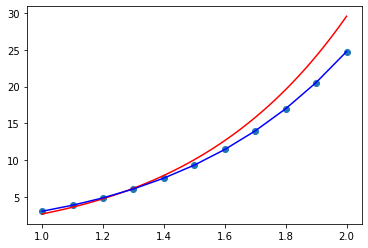
\includegraphics[scale=0.75]{4-2shooting}
\end{center}

Конечно-разностный метод
\begin{center}
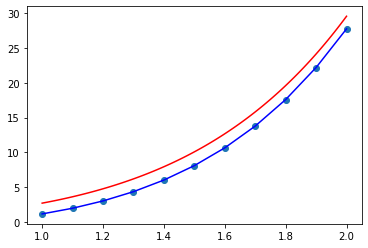
\includegraphics[scale=0.75]{4-2fin-dif}
\end{center}
\pagebreak

\subsubsection{Исходный код}
\lstinputlisting{../lab4_2/boundary_solver.hpp}
\pagebreak
